%% LaTeX-Beamer template for KIT design
%% by Erik Burger, Christian Hammer
%% title picture by Klaus Krogmann
%%
%% version 2.1
%%
%% mostly compatible to KIT corporate design v2.0
%% http://intranet.kit.edu/gestaltungsrichtlinien.php
%%
%% Problems, bugs and comments to
%% burger@kit.edu

\documentclass[18pt]{beamer}
\usepackage[utf8x]{inputenc}
\usepackage{units}
\usepackage{booktabs}

%% CUSTOM
\usepackage{amsmath}
\usepackage{algpseudocode}

%% Definitions
\DeclareMathOperator{\div2}{div}
\renewcommand{\algorithmicrequire}{\textbf{Input:}}
\renewcommand{\algorithmicensure}{\textbf{Output:}}
\algnewcommand\algorithmicto{\textbf{to}}
\algrenewtext{For}[3]{\algorithmicfor\ $#1 \gets #2$ \algorithmicto\ $#3$ \algorithmicdo}
\algnewcommand\algorithmicod{\textbf{od}}
\algrenewtext{EndWhile}{\algorithmicod}
\algrenewtext{EndFor}{\algorithmicod}
%\AtBeginSection[]{%
%\begin{frame}<beamer> % do nothing in handouts
%    \frametitle{Überblick}
%    \tableofcontents[sectionstyle=show/shaded,
%    subsectionstyle=show/show/hide]
%\end{frame}
%}
%\AtBeginSubsection[]{%
%\begin{frame}<beamer> % do nothing in handouts
%    \frametitle{Überblick}
%    \tableofcontents[sectionstyle=show/shaded,
%    subsectionstyle=show/shaded/hide]
%\end{frame}
%}

%% SLIDE FORMAT

% use 'beamerthemekit' for standard 4:3 ratio
% for widescreen slides (16:9), use 'beamerthemekitwide'

\usepackage{templates/beamerthemekit}
%\usepackage{templates/beamerthemekitwide}

 %% TITLE PICTURE

 % if a custom picture is to be used on the title page, copy it into the 'logos'
 % directory, in the line below, replace 'mypicture' with the 
 % filename (without extension) and uncomment the following line
 % (picture proportions: 63 : 20 for standard, 169 : 40 for wide
 % *.eps format if you use latex+dvips+ps2pdf, 
 % *.jpg/*.png/*.pdf if you use pdflatex)


 \titleimage{banner}
 
 
%% Define some colors:
\definecolor{darkblue}{rgb}{0,0,.5}
\definecolor{darkgreen}{rgb}{0,.5,0}

 %% TITLE LOGO

 % for a custom logo on the front page, copy your file into the 'logos'
 % directory, insert the filename in the line below and uncomment it

\titlelogo{logo_150x150}
 
 % (*.eps format if you use latex+dvips+ps2pdf,
 % *.jpg/*.png/*.pdf if you use pdflatex)
 
 %% TikZ INTEGRATION
 
 % use these packages for PCM symbols and UML classes
 % \usepackage{templates/tikzkit}
 % \usepackage{templates/tikzuml}
 
 % the presentation starts here
 
\author{Dominik Muth - dominik.muth@student.kit.edu}
\institute{Institut f\"ur Informatik}


\title[Tutorium 8]{GBI Tutorium Nr. $2^5$}
\subtitle{Tutorium 8}
\date{12. Dezember 2012}

% Bibliography



\begin{document}

	%title page
	\begin{frame}
		\titlepage
	\end{frame}

	%table of contents
	\begin{frame}{Outline/Gliederung}
		\tableofcontents
	\end{frame}
	
	
	\begin{frame}
		\begin{block}{Hinweis}
			\begin{itemize}
				\item Habt ihr euch für den Übungsschein angemeldet?
				\pause
				\item Und für die Klausur?
			\end{itemize}
		\end{block}
	\end{frame}
	
		
	
	
	
	\section{Wiederholung} 
	\begin{frame} {Wiederholung - Quiz}
		\begin{itemize}
			\item Zwei unterschiedliche Graphen können das gleiche Aussagen.
			\only<2-> {\color{darkgreen}$\surd$}\\
			\color{black}
					
			\item Ein Teilgraph ist definiert mit $V' \subseteq V, E' \subseteq V' \times V'$
			\only<3-> {\color{red}$X$}\\
			\color{black}
	
			\item In jedem gerichteten Baum gibt es genau einen Knoten $x_0$ mit
$d^{+}(x_0) = 0 \land d^{−}(x_0) \geq 0$
			\only<4-> {\color{darkgreen}$\surd$}\\
			\color{black}
			
			\item Zwischen zwei isomorphen Graphen gibt es immer nur einen Isomorphismus
			\only<4-> {\color{red}$X$}\\
			\color{black}
		\end{itemize}
	\end{frame}
	
	
	
	\begin{frame} {Wiederholung - Aufgaben}
		\begin{block}{Isomorphie}
			Geben Sie alle Isomorphismen zwischen $G_0$ und $G_1$ an.
			\begin{center}
				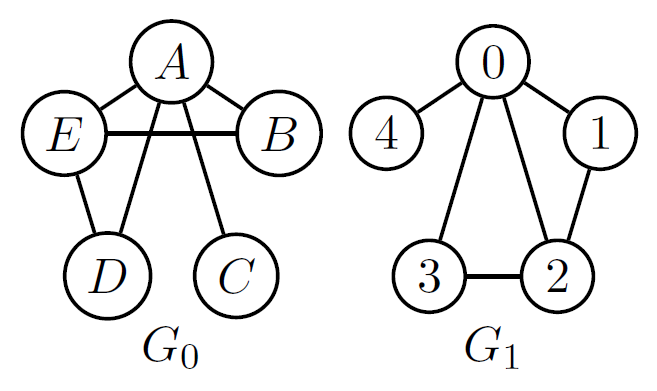
\includegraphics[scale=0.4]{graphics/08/isomorphie.png}
			\end{center}					 
		\end{block}
	\end{frame}
	
	
	
	\begin{frame} {Wiederholung}
		\begin{block} {Graphen: ÜB7 (WS08/09)}
			Gegeben sei der Graph $G = (V,E)$ mit $V = \{0,1\}^3$ und $E = \{(xw, wy)\;|\;x,y \in \{0,1\} \land w \in \{0,1\}^2\}$.
			
			\begin{itemize}
				\item Zeichen Sie den Graphen
				\item Geben Sie einen Zyklus in G an, der außer dem 
					Anfangs- und Endknoten jeden Knoten von G genau einmal enthält.
				\item Geben Sie einen geschlossenen Pfad in G an, 
					der jede Kante von G genau einmal enthält.
			\end{itemize}
		\end{block}
	\end{frame}
	
	
	\section{Graphen im Rechner}
	\begin{frame}{Graphen im Rechner}
		\begin{itemize}
			\item Wie werden Graphen gespeichert?
			\item Wie "effizient" sind die Methoden?
			\item Was verstehen wir unter Effizienz?
		\end{itemize}
	\end{frame}
	
	
	\subsection{Adjazenzmatrix}
	\begin{frame}{Adjazenzmatrix}
		\begin{block}{Was ist das?}
			Ein Graph kann in einer $n \times n$ Matrix gespeichert werden, 
			wobei gilt: $n = |V|$.\\
			\vspace{10pt}
			\pause
			Wie kann man sich dies Vorstellen?\\
			\pause
			Für jede Kante $(x,y)$ existiert eine 1 in der Matrix an der stelle $(x,y)$.
		\end{block}
		
		\visible<4->{
		\begin{exampleblock}{Beispiel}
			Wie sieht die Adjazenzmatrix für folgenden gerichteten Graphen aus:\\
			$G = (V, E)$\\
			$V = \{0,1,2,3,4\}$\\
			$E = \{(0,0), (0,1), (0,2), (0,4), (2,3), (4,1), (2,0)\}$
		\end{exampleblock}
		}
	\end{frame}
	
	
	\begin{frame}{Adjazenzmatrix}
		Einige Denkanstöße:
		\begin{itemize}
			\pause
			\item Wie sieht es mit dem Speicherplatz aus?
			
			\pause
			\item Wie ''schnell'' kann man herausfinden, ob eine Kante zwischen x und y existiert?
			
			\pause
			\item Wie schnell hat man Zugriff auf alle adjazenten Knoten von einem Knoten x?
			
			\pause
			\item Woran erkennt man Schlingen?
			
			\pause
			\item Welche Eigenschaft haben Adjazenzmatrizen ungerichteter Graphen?
		\end{itemize}
	\end{frame}
	
	
	\begin{frame}{Aufgabe}
		\begin{block}{}
			Gegeben sei folgende Adjazenzmatrix:\\
			A = $\kbordermatrix{
          		  & 0 & 1 & 2 & 3 \\
        		0 & 0 & 1 & 0 & 1 \\
        		1 & 0 & 0 & 0 & 0 \\
        		2 & 0 & 0 & 1 & 1 \\
        		3 & 0 & 0 & 1 & 0 \\
      			}$\\
      		\vspace{10pt}
      		Zeichen Sie den Graphen zur Adjazenzmatrix A.
		\end{block}
		
	\end{frame}
	
	
	
	\subsection{Adjazenzliste}
	\begin{frame}{Adjazenzliste}
		\begin{block}{Was ist das?}
			Bei einer Adjazenzliste wird für jeden Knoten einzeln gespeichert, welche ausgehenden Kanten dieser besitzt.
		\end{block}
		
		\begin{exampleblock}{Beispiel}
			Wie sieht die Adjazenzliste für den Graphen von vorhin aus:\\
			$G = (V, E)$\\
			$V = \{0,1,2,3,4\}$\\
			$E = \{(0,0), (0,1), (0,2), (0,4), (2,3), (4,1), (2,0)\}$
		\end{exampleblock}
	\end{frame}
	
	
	\begin{frame}{Adjazenzliste}
		Nochmal Denkanstöße:
		\begin{itemize}
			\pause
			\item Wie sieht es mit dem Speicherplatz aus?
			
			\pause
			\item Wie ''schnell'' kann man herausfinden, ob eine Kante zwischen x und y existiert?
			
			\pause
			\item Wie schnell hat man Zugriff auf alle adjazenten Knoten von einem Knoten x?
			
			\pause
			\item Sind Adjazenzlisten besser als Adjazenzmatrizen?
			
		\end{itemize}
	\end{frame}
	
	
	\begin{frame}{Aufgabe}
		\begin{block}{}
			Zeichnen sie den Graphen zur folgenden Adjazenzliste:\\
			\begin{center}
				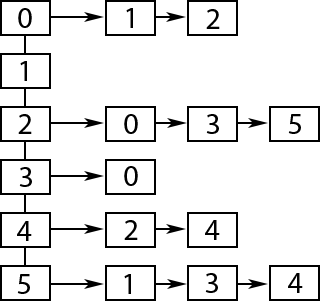
\includegraphics[scale=0.5]{graphics/08/adjazenzliste.png}
			
			\end{center}
		\end{block}
	\end{frame}
	
	
	\subsection{Wegematrix}
	\begin{frame}{Wegematrix}
		\begin{block}{Wozu?}
			Die Wegematrix sagt uns, ob ein Pfad zwischen zwei Knoten existiert.
		\end{block}
		
		\begin{exampleblock}{Beispiel}
			Zeichnen Sie die Wegematrix zum Graphen, der an der Tafel stehen sollte.
		\end{exampleblock}
	\end{frame}
	
	
	\begin{frame}{Wegematrix}
		\begin{itemize}
			\item Wie sieht die Wegematrix aus, wenn $A$ = alles Eins?\\
			\color{darkgreen}\visible<2->{W = A}\color{black}
			
			\item \visible<3-> {Wann ist allgemein W = A?}\\
			\color{darkgreen}\visible<4->{Wenn Kantenrelationen reflexiv und transitiv}\color{black}
			
			\item \visible<5-> {Warum nicht symmetrisch?}\\
			\color{darkgreen}\visible<6-> {Auch Wegematrizen können asymmetrisch sein.}\color{black}
		\end{itemize}
	\end{frame}
	
	
	\subsection{2-Erreichbarkeitsrelation}
	\begin{frame}{2-Erreichbarkeitsrelation}
		\begin{block}{Was ist das?}
			Über die 2-Erreichbarkeitsrelation können wir herausfinden, welche Knoten über 2 Kanten erreichbar sind.
		\end{block}
		
		\pause
		\begin{block}{Wie gehts das?}
			Indem wir die Adjazenzmatrix mit sich selbst mal nehmen. ($A^2$)
		\end{block}
	\end{frame}
	
	
	\begin{frame}{Einschub - Matrixmultiplikation}
		\begin{block}{Definition}
			Wir definieren $x_{ij}$ als das Element der Matrix X, 
			welches in der i-ten Zeile und j-ten Spalte.\\
			
			Dann lässt sich die Multiplikation der Matrizen A und B 
			folgendermaßen darstellen:\\
		
			\[\forall c \in C \;|\; c_{ij} = \sum_{k=1}^m a_{ik} \cdot b_{kj}\]\\
			mit $b\in B, a\in A$ und $m$ sei die Breite der Matrix A 
			und die Höhe der Matrix B.
		
		\end{block}
	\end{frame}
	
	\begin{frame}{Einschub - Matrixmultiplikation}
		\begin{exampleblock}{Beispiel}
			\[\begin{pmatrix}
    			1 & 2 & 3 \\
    			4 & 5 & 6 \\
  			\end{pmatrix}
  			\cdot
  			\begin{pmatrix}
    			6 & -1 \\
    			3 & 2 \\
    			0 & -3
 			 \end{pmatrix}
  			=\]\\
  			\[
  			\begin{pmatrix}
     			1 \cdot 6  +  2 \cdot 3  +  3 \cdot 0 &
     			1 \cdot (-1) +  2 \cdot 2 +  3 \cdot (-3) \\
     			4 \cdot 6  +  5 \cdot 3  +  6 \cdot 0 &
     			4 \cdot (-1) +  5 \cdot 2 +  6 \cdot (-3) \\
  			\end{pmatrix}
  			=
  			\begin{pmatrix}
    			12 & -6 \\
    			39 & -12
  			\end{pmatrix}\]
		\end{exampleblock}
	\end{frame}
	
	
	\begin{frame}{2-Erreichbarkeitsrelation}
		\begin{block}{Was ist das?}
			Über die 2-Erreichbarkeitsrelation können wir herausfinden, welche Knoten über 2 Kanten erreichbar sind.
		\end{block}
		
		\begin{block}{Wie gehts das?}
			Indem wir die Adjazenzmatrix mit sich selbst mal nehmen. ($A^2$)
		\end{block}
		
		\begin{block}{Warum funktioniert das?}
			siehe Beispiel an der Tafel		
		\end{block}
	\end{frame}
	
	\begin{frame}{Aufgaben}
	\end{frame}
	
	
	\begin{frame}{Wegematrix}
		Wie können wir die 2-Erreichbarkeitsrelation also nutzen, um die Wegematrix aufzustellen?\\
		\vspace{10pt}
		\pause
		Geht es auch einfacher/schneller?
	\end{frame}
	
	
	
	\subsection{Algorithmus von Warshall}
	\begin{frame}{Algorithmus von Warshall}
		\begin{block}{Definition}
			Der Warshall-Algorithmus ist ein Algorithmus zum Berechnen von Wegematrizen.
		\end{block}
		
		\begin{block}{Algorithmus Teil 1}
            \begin{algorithmic}
				\For{i}{0}{n-1}
					\For{j}{0}{n-1}
						\If{$i = j$}
							\State $W[i,j] \gets 1$;
						\Else
							\State $W[i,j] \gets A[i,j]$
						\EndIf
					\EndFor
				\EndFor
            \end{algorithmic}
			
		\end{block}
	\end{frame}
	
	
	\begin{frame}{Algorithmus von Warshall}
	
		
		\begin{block}{Algorithmus Teil 2}
            \begin{algorithmic}
				\For{k}{0}{n-1}
					\For{i}{0}{n-1}
						\For{j}{0}{n-1}
							\State $W[i , j ] \gets  max(W[i , j ]; min(W[i , k];W[k, j ]) )$
						\EndFor
					\EndFor
				\EndFor
            \end{algorithmic}
			
		\end{block}
		
		\begin{exampleblock}{Beispiel}
			$G = (\{0,1,2,3\}, \{(0,3), (1,0), (2,3), (3,1)\})$
		\end{exampleblock}
	\end{frame}
	
	
	\begin{frame}{Aufgabe}
		\begin{block}{}
			Gegeben sei eine Adjazenzliste, bilden Sie die Adjazenzmatrix und bestimmen Sie mit Hilfe des Warshall-Algorithmus die Wegematrix.\\
			
		\begin{center}
			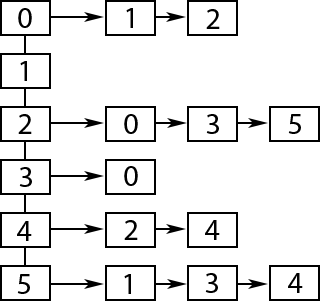
\includegraphics[scale=0.5]{graphics/08/adjazenzliste.png}
		\end{center}
			
		\end{block}
	\end{frame}
	
	
	\section{Fragen}
	\begin{frame} {Fragen}
		\begin{itemize}
			\item Fragen zum Stoff?
			\item Fragen zum n\"achsten \"Ubungsblatt?
			\item Generelle Fragen?
			\item Feedback?
		\end{itemize}
	\end{frame}

		
	\begin{frame} {EOF}
		\begin{center}
			
\includegraphics[scale=0.45]{graphics/eof8.png}\\
			\tiny $source: http://imgs.xkcd.com/comics/porn.png$
		\end{center}
	\end{frame}

\end{document}
